%% LyX 2.0.5.1 c	reated this file.  For more info, see http://www.lyx.org/.
%% Do not edit unless you really know what you are doing.
\documentclass[11pt,oneside,final]{fithesis2}
%\usepackage[total={30em	,23cm}, includefoot]{geometry}

%% Basic packages
\usepackage[czech]{babel}
\usepackage{cmap}
\usepackage[T1]{fontenc}
\usepackage{lmodern}
\usepackage[utf8]{inputenc}
\usepackage{graphicx}

%% Additional packages for colors, advanced
%% formatting options, etc.
\usepackage{color}
\usepackage{microtype}
\usepackage{url}
\usepackage{cslatexquotes}
\usepackage{fancyvrb}
\usepackage[small,bf]{caption}
\usepackage[plainpages=false,pdfpagelabels,unicode]{hyperref}
\usepackage[all]{hypcap}

\languageattribute{czech}{split}
\usepackage{cite}
\setcounter{secnumdepth}{3}
\setcounter{tocdepth}{3}
\usepackage{hanging}
\usepackage{listings}
\usepackage{comment}
\usepackage{textcomp}
\definecolor{listinggray}{gray}{0.9}
\definecolor{lbcolor}{rgb}{0.9,0.9,0.9}
\usepackage{zref-user}
\renewcommand{\baselinestretch}{1.13}

\newcommand\todo[1]{\noindent\textcolor{red}{#1}}
\newcommand\nove[1]{\textcolor{green}{#1}}


\lstset{
	%backgroundcolor=\color{lbcolor},
	tabsize=4,
	rulecolor=,
        basicstyle=\scriptsize,
        upquote=true,
        aboveskip={1.5\baselineskip},
        columns=fixed,
        showstringspaces=false,
        extendedchars=true,
        breaklines=true,
        prebreak = \raisebox{0ex}[0ex][0ex]{\ensuremath{\hookleftarrow}},
        frame=single,
        showtabs=false,
        captionpos=b, 
        showspaces=false,
        showstringspaces=false,
        identifierstyle=\ttfamily,
        keywordstyle=\color[rgb]{0,0,1},
        commentstyle=\color[rgb]{0.133,0.545,0.133},
        stringstyle=\color[rgb]{0.627,0.126,0.941},
        extendedchars=true,
        inputencoding=utf8,
    extendedchars=true,
    literate=%
    {á}{{\'a}}1
    {č}{{\v{c}}}1
    {ď}{{ \v{d}}}1
    {é}{{\'e}}1
    {ě}{{\v{e}}}1
    {í}{{\'i}}1
    {ň}{{\v{n}}}1
    {ó}{{\'o}}1
    {ř}{{\v{r}}}1
    {š}{{\v{s}}}1
    {ť}{{\v{t}}}1
    {ú}{{\'u}}1
    {ů}{{\r{u}}}1
    {ý}{{\'y}}1
    {ž}{{\v{z}}}1
    {Á}{{\'A}}1
    {Č}{{\v{C}}}1
    {Ď}{{\v{D}}}1
    {É}{{\'E}}1
    {Ě}{{\v{E}}}1
    {Í}{{\'I}}1
    {Ň}{{\v{N}}}1
    {Ó}{{\'O}}1
    {Ř}{{\v{R}}}1
    {Š}{{\v{S}}}1
    {Ť}{{\v{T}}}1
    {Ú}{{\'U}}1
    {Ů}{{\r{U}}}1
    {Ý}{{\'Y}}1
    {Ž}{{\v{Z}}}1   
}

\definecolor{darkgray}{rgb}{.4,.4,.4}
 
\lstdefinelanguage{AspectJ}[]{Java}{
    morekeywords={declare, pointcut, aspect, before, around, after, returning, throwing, call, execution, this, target, args, within, withincode, get, set, initialization, preinitialization, staticinitialization, handler, adviceexecution, cflow, cflowbelow, if, proceed},
    moredelim=[is][\textcolor{darkgray}]{\%\%}{\%\%},
    moredelim=[il][\textcolor{darkgray}]{§§}
}

\makeatletter
\renewcommand{\@chapapp}{}% Not necessary...
\newenvironment{chapquote}[2][2em]
  {\setlength{\@tempdima}{#1}%
   \def\chapquote@author{#2}%
   \parshape 1 \@tempdima \dimexpr\textwidth-2\@tempdima\relax%
   \itshape}
  {\par\normalfont\hfill--\ \chapquote@author\hspace*{\@tempdima}\par\bigskip}
\makeatother

%% Fix long URLs in DVIs
\usepackage{ifpdf}
\ifpdf
\else
  \usepackage{breakurl}
\fi

%% Packages used to generate various lists
\usepackage{makeidx}
\makeindex

\usepackage[xindy]{glossaries}
\makeglossary
 
\thesistitle{Srovnání RAD~platforem Seam~Forge a~Spring~Roo} % enter thesis title
\thesissubtitle{Bakalářská práce}
\thesisstudent{Jan Holman} % name of the author
\thesiswoman{false} % defines author’s gender
\thesisuniversity{Masarykova univerzita}
\thesisfaculty{Fakulta informatiky}
\thesislogo{fi-logo}
\thesisyear{Brno, jaro 2013}
\thesisadvisor{Mgr. Marek Grác, Ph.D.} % fill in advisor’s name
\thesislang{cs} % thesis is in Czech

%% Beginning of the document
\begin{document}

%% Front page with a logo and basic thesis information
\FrontMatter
\ThesisTitlePage

%% Thesis declaration (required)
\begin{ThesisDeclaration}
  \DeclarationText
  \AdvisorName
\end{ThesisDeclaration}


%% Thanks (optional)
\begin{ThesisThanks}

\end{ThesisThanks}


%% Abstract (required)
\begin{ThesisAbstract}

\end{ThesisAbstract}

%% Keywords (required)
\begin{ThesisKeyWords}

\end{ThesisKeyWords}

%% Beginning of the thesis itself
\MainMatter

%% TOC (required)
\tableofcontents

%% Thesis text structured using
%% chapters, sections, subsections, etc.
\chapter{Úvod} 
\section{Cíle práce}
\section{Struktura práce}

\chapter{Rapid Application Development}
\begin{chapquote}{The Mustard Seed Garden Manual of Painting}
Some consider it noble to have a method; others consider it noble 
not to have a method. Not to have a method is bad; to stop entirely 
at method is still worse. One should at first observe rules severely, 
then change them in an intelligent way. The aim of possessing 
method is to seem finally as if one had no method.
\end{chapquote}

Rapid Application Development, v překladu \uv{rychlý vývoj aplikací} je metodologie tvorby (mj.) softwaru, která, jak už název napovídá, upřednostňuje rychlost vytváření funkčních prototypů tradičně na úkor použitelnosti, rozsahu implementovaných funkcí a / nebo výkonu. RAD také značně omezuje část plánování ve prospěch samotného vývoje, který probíhá iterativně. Důraz se klade na tvorbu prototypů, na aktivní komunikaci s klientem a jeho participaci na vývoji \todo{citace}. Metoda byla poprvé popsána v roce 1991 Jamesem Martinem v knize Rapid Application Development jako reakce na tehdejší metody vývoje, které zejména nedokázaly dostatečně pružně reagovat na změny požadavků v průběhu vývoje, a na základě potřeby dodat co nejrychleji fungující systém.\cite{BlueInk} 

\section{Rozdíly oproti jiným metodám}
Hlavní problém tehdy nejrozšířenější metody tzv. vodopádu je ten, že vývoj systému trvá příliš dlouho. V průběhu vleklého vývoje se mohou klientovy potřeby změnit, takže výsledkem je sice kompletní a technicky dokonalý ale zároveň nepoužitelný systém. Čím déle vývoj trvá, tím vyšší je pravděpodobnost změny v požadavcích, a na tyto změny je třeba pružně reagovat.
Oproti běžným agilním metodám se RAD soustředí na vývoj pro uživatele nejzajímavějších částí \todo{(?)} – vychází z předpokladu, že uživatelé nejčastěji využívají funkce, které jsou pro ně zajímavé, a proto mají tyto části vyšší prioritu. \todo{citace} RAD také klade důraz na co nejrychlejší naplnění potřeby klienta, spíš než na technickou a technologickou dokonalost. 
Hlavní oblasti, ze kterých plyne rychlost vývoje pomocí RAD jsou prototypování, iterace a tzv. timeboxing.\\
Prototypování spočívá v co možná nejrychlejší vytvoření fungujícího prototypu (řádově v jednotkách dní), který se zaměřuje pouze na klíčové funkce, a v jeho následném ladění na základě odezvy od klienta a budoucích uživatelů. Nejde pouze o jednorázové prototypy, jako u jiných agilních metod (\todo{např.}), celý software vzniká iterativně postupným rozšiřováním prvotního prototypu. Prototyp slouží jako důkaz práce pro klienta (například při vývoji pomocí vodopádu klient velmi dlouho nevidí žádný nebo minimální výstup) a také jako referenční bod, ze kterého se vychází při dalším zpřesňování požadavků. Rychlé tvorby prvního prototypu se dosahuje využíváním tzv. CASE \todo{odkaz dolů} nástrojů, které z formálního zápisu požadavků automaticky generují datový model, funkční databázi a aplikační kód.\\
Podle pravidla timeboxingu je nutné dodávat výsledky každé iterace včas, a to i za cenu, že se část nestihne a přesune se do dalšího cyklu. Je lepší dodat část zadání včas, než dodat všechno, ale nedodržet časový plán. Pokud by se jednotlivé cykly protahovaly, omezovala by se odezva od klienta a metoda by tím ztrácela podstatnou část výhod z plynoucích z iterativního vývoje.\\
Během vytváření modelu i celého iteračního procesu jsou také aktivně zapojeni uživatelé/klient, kteří se podílejí na návrhu a schvalují prototypy. 

\section{Fáze vývoje pomocí RAD}
\begin{figure}[h!]
  \centering
    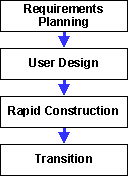
\includegraphics[scale=0.8]{img/rad-phases.png}
    \caption{Fáze RAD\cite{RAD1}}
\end{figure}

\begin{enumerate}
\item Plánování požadavků: Definování funkcí, procesů, dat a rozsahu sytému. Výsledkem je seznam entit a diagramů, které definují interakce mezi procesy a datovými elementy. Zachycení požadavků v nástroji tak, aby se daly později automaticky převést na datový model a kód (ne pouze v nestrukturovaném dokumentu).
\item Uživatelský návrh: Workshopy s uživateli/klientem, modelování dat a procesů systému, vytvoření funkčního prototypu kritických částí systému. Detailní rozvedení požadavků a převedení definovaných entit na datový model, formalizování pravidel, tvorba testovacích plánů, návrh obrazovek uživatelského rozhraní a vazeb mezi nimi. Odhad náročnosti vývoje daného systému, vytvoření prvního omezeného prototypu, který se zaměřuje pouze na (předem definované) klíčové funkce, pomocí CASE nástrojů.
\item Rychlý vývoj: Vlastní tvorba samotného aplikačního systému, tvorba uživatelské podpory a implementace pracovních plánů. Vývoj probíhá v krátkých cyklech - vývoj, testování, upřesnění požadavků, další cyklus (s využitím principu timeboxingu). Převod datového modelu na funkční databázi. 
\item Nasazení: Akceptační testování, školení uživatelů, konverze dat, nasazení systému do podniku.\cite{RAD-pdf}
\end{enumerate}

\section{Výhody}
Hlavní výhody plynoucí z RAD jsou rychlost a kvalita. Rychlost je zde dána krátkou dobou mezi dodávkami v jednotlivých cyklech, především díky využívání CASE nástrojů, které ve velmi krátkém čase konvertují požadavky na kód, a principu timeboxingu, tedy striktního dodržování časového plánu. Kvalita se v případě RAD nechápe v tradičním (a asi intuitivnějším) významu, tedy ve smyslu míry, do jaké výsledný systém splňuje zadané požadavky, a míry, do jaké v něm po dodání nedochází k závadám, ale spíš se chápe jako míra, do jaké systém naplňuje potřeby klienta a do jaké má malé náklady na údržbu. Vysoké kvality se v případě RAD dosahuje pomocí aktivního zapojené budoucích uživatelů do celého procesu tvorby systému, především ve fázích analýzy a návrhu.\cite{BlueInk}

\section{Nevýhody}
Problémy, které mohou při vývoji pomocí RAD potenciálně vzniknout, jsou především horší škálovatelnost a omezený rozsah vytvořeného systému. Protože při vývoji nejprve vzniká jednoduchý prototyp, který se později iterativně rozvíjí do kompletní aplikace, může výsledek škálovat hůř, než řešení, které je od počátku navržené jako kompletní aplikace.
Výsledná aplikace může také vlivem timeboxingu, tedy upřednostňováním včasného doručení před implementováním všech slíbených funkcí, obsahovat méně funkcí, než aplikace vytvořená tradičním způsobem (například metodou vodopádu).\\
RAD se samozřejmě nedá použít na všechny typy projektů – například systém řízení letadla vytvořený pomocí RAD by asi moc důvěry nevzbuzoval. Tento přístup je vhodný zejména pro menší projekty, nebo pro projekty, u kterých lze práci rozdělit na více zvládnutelných částí. Stejně tak by měl být poměrně malý i vývojářský tým (ideálně 2-6 lidí) a jeho členové by s tímto typem vývoje měli mít zkušenosti. Nutnou podmínkou jsou dobře definované požadavky a rozsah vytvářené aplikace, malé množství rozhodujících na straně klienta (ideálně 1 člověk) a jejich jasně určení.\cite{BlueInk} 

\section{Nástroje podporující metodu RAD}
Důležitou součástí vývoje pomocí RAD je využívání kvalitních nástrojů podporujících rychlý vývoj, tedy především CASE nástrojů, které generují aplikační kód. Bohužel ne všechny nástroje, které o sobě prohlašují, že podporují rychlý vývoj, jsou pro metodu RAD skutečně vhodné. Použité nástroje by měly umět strukturovaně zachytit požadavky (UML \todo{odkaz dolů} nástroje), převést zachycené požadavky na datový model a na jeho základě vygenerovat funkční databázi a velkou část aplikačního kódu.\\
Základní požadavky na kvalitní nástroj podporující RAD\cite{BlueInk} :
\begin{itemize}
  \item produkuje kód na úrovni enterprise (n-tier) \todo{?}
  \item generuje kompletní prvotní prototyp bez nutnosti přímého psaní kódu (vč. prezentační vrstvy)
  \item umožňuje plnou kontrolu nad generovaným kódem, například pomocí šablon
  \item poskytuje flexibilní systém metadat \todo{?}
  \item dá se použít během celého vývoje a zejména nepřepíše kód vývojáře
\end{itemize}

\url{http://en.wikipedia.org/wiki/List_of_graphical_user_interface_builders_and_rapid_application_development_tools}

\section{Spring Roo}
Spring Roo je textový open source nástroj usnadňující vývoj podnikových aplikací. Je plně založený na jazyce Java EE a využívá běžné a osvědčené knihovny a rámce, jako jsou standardy Bean Validation (JSR-303) a Dependency Injection (JSR-330), a splňuje osvědčené praktiky aplikační architektury SpringSource. Aplikace vytvořené pomocí Roo využívají principu \uv{convention over configuration}, což znamená, že se vývojář musí se musí explicitně starat jen o ty části, které v daném projektu neodpovídají běžným konvencím. V ostatních případech je vše automaticky nakonfigurováno podle konvencí dané technologie.\cite{Roo}\\
Nástroj byl poprvé uveden v květnu 2009 na vývojářské konferenci SpringOne Europe a od té doby se kolem něj vytvořila silná komunita uživatelů, kteří si vzájemně radí na fóru a vytvářejí pro Roo další uživatelská rozšíření.\cite{Roo-clanek}\\
Roo pyšní svou schopností významně zvýšit produktivitu vývojářů tím, že nabízí abstrakci nad technologiemi, jako je rámec Spring Framework, Java Persistence API, JavaServer Pages, Spring Security, Spring Web Flow, Log4J nebo Maven, a výrazně snižuje čas a úsilí potřebné k použití těchto technologií v projektu. S Roo není třeba se nic učit nebo vytvářet vlastní řešení a "znovu vynalézat kolo", stačí zadat příkaz a Roo danou technologii do projektu přidá, nakonfiguruje a potom automaticky spravuje příslušné soubory (konfigurační \textit{xml} a \textit{properties} soubory, jsp stránky..). Roo navíc maximalizuje využití stávajících znalostí a zkušeností vývojáře, který používané technologie už v mnoha případech zná.\\
Nástroj Spring Roo se především hodí k rychlému vytváření CRUD \footnote{CRUD aplikace - Jednoduchá aplikace, která umožňuje vytvoření, čtení, editaci a smazání záznamů v trvalém úložišti} aplikací a prototypů, k automatickému přidání a konfiguraci určité technologie, případně ho lze dobře využít k učení se nových technologií pomocí snadno vytvořené fungující aplikace, která danou technologii využívá.\cite{Roo-clanek}\\

Typická aplikace vytvořená pomocí Spring Roo se neliší od většiny podnikových aplikacích napsaných v jazyce Java – obsahuje relační databázi, přístup pomocí JPA\footnote{Java Persistence API}, Spring Framework dependency injection a správu transakcí, testování pomocí knihovny JUnit, k sestavení využívá systém Maven a obvykle obsahuje prezentační vrstvu založenou na modelu Spring MVC\footnote{Model View Controler}, která využívá JSP\footnote{JavaServer Pages} stránky.\\
Technologie jsou přidávány inkrementálně na požádání, takže projekt není zatížen žádnými nepotřebnými závislostmi nebo konfiguračními soubory.\\

Celkový pohled na práci Roo nad projektem je vidět na následujícím obrázku:\\
\begin{figure}[h!]
  \centering
    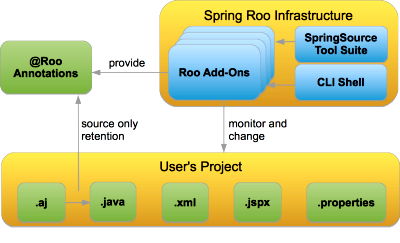
\includegraphics[scale=0.8]{img/roo-architektura.png}
    \caption{Schéma fungování Spring Roo nad projektem\cite{RooPDF}}
\end{figure}
Spring Roo ve formě addonů (buď jako samostatný nástroj v shell příkazové řádce, nebo jako součást balíku SpringSource Tool Suite) vytváří a sleduje změny v uživatelských souborech, přidává anotace začínající na \textit{@Roo} do kódu a udržuje tak vazbu mezi java třídami (\textit{.java}) a deklaracemi AspectJ (\textit{.aj}).

Roo nedokáže vytvořit vlastní logickou vrstvu systému, ale postará se o infrastrukturu a konfiguraci aplikace. Lze ho použít k vytvoření nového projektu i k přidání určité funkcionality do již existujícího projektu. Na rozdíl od podobných nástrojů neposkytuje pomoc jen na začátku projektu, ale sleduje průběh celého vývoje, po celou dobu se stará o části projektu a sleduje změny.

\subsection{Odstranění z projektu}
Existují rizika, kvůli kterým může vývojář chtít přestat Roo používat – např. se změní požadavky, objeví se vhodnější alternativa, nástroj může obsahovat neúnosné množství chyb, nemusí podporovat potřebné verze softwaru atd. V tom případě je velkou výhodou fakt, že Spring Roo nijak neovlivňuje běh vznikající aplikace a je ho tedy možné "beztrestně" odstranit. Běh aplikace se tím nijak neovlivní. Veškerá funkcionalita Roo je využívána během vývoje a sestavené aplikace se nijak nedotýká - anotace @Roo slouží pouze k udržování informací o zdrojovém kódu a při kompilaci jsou odstraněny. Proto Roo nemá vliv ani na výkon a paměťové nároky výsledného systému.\\
Odstranění Roo trvá několik minut a zahrnuje pouze \todo{refactor} kódu a jednoduché vyhledání a nahrazení klíčových slov. Celý proces je popsán v dokumentaci\cite{RemovingRoo} a existuje k němu mnoho demonstrací.\\
Díky snadnému odstranění nástroje z projektu nedochází ani k proprietárnímu uzamčení, tedy vytvoření závislosti na jednom konkrétním nástroji nebo společnosti.

\subsection{Použitelnost}
Nástroj Spring Roo je většinou spouštěn ve zvláštním okně mimo používané IDE nebo textový editor a nevyžaduje pozornost ze strany uživatele. Místo toho běží na pozadí a monitoruje změny v projektu. Ani změny, provedené v době, kdy Roo neběží, nejsou problémem, protože Roo při každém spuštění projde všechny soubory a vyhledá případné změny.\\
Nástroj klade velký důraz na použitelnost a jeho uživatelské rozhraní (příkazový řádek) je inspirováno knihou Jefa Raskina \textit{The Humane Interface}. Podle zásad v ní popsaných se snaží neomezovat uživatele v tom, co chce zrovna udělat, a nenarušovat jeho soustředění, ale naopak předvídat akce z jeho strany a korektně na ně reagovat.\\
Roo se také snaží o to, aby byla doba potřebná k naučení se práce s ním co možná nejkratší. Toho dosahuje několika způsoby:
\begin{itemize}
\item používá standardní Java technologie, u kterých je vysoká šance, že je uživatel již zná,
\item běží na pozadí a nevyžaduje pozornost uživatele, pokud to sám nepotřebuje zadávat příkazy a provádět změny,
\item zahrnuje funkce usnadňující učení, jako je doplňování příkazů po stisknutí tabulátoru nebo kontextová nápověda ve formě příkazu \uv{hint}, který na základě stavu projektu a nedávné aktivity uživatele navrhuje další možný postup,
\item řídí se jasně definovanými konvencemi\cite{Roo-konvence},
\item pracuje v \uv{bezpečném režimu}, takže se všechny změny provedené pomocí něj dají zvrátit díky automatickému roll-backu
\end{itemize}

\subsection{AspectJ}
\begin{figure}[h!]
  \centering
    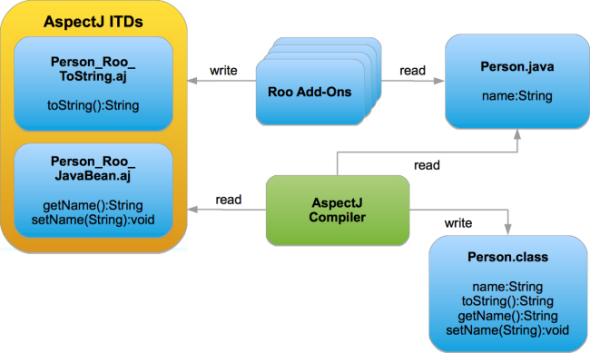
\includegraphics[scale=0.8]{img/roo-aspectj.png}
    \caption{AspectJ ITD\cite{RooPDF}}
\end{figure}

Jak je u Springového nástroje dá očekávat\cite{Roo-AspectJ}, i Spring Roo je z velké části založen na technologii AspectJ – konkrétně na výhodách plynoucích z možností ITD\footnote{inned type declaration}. Metody, které generuje a spravuje Roo, nejsou obsažené přímo ve zdrojových \textit{.java} souborech, ale v externích ITD souborech s příponou \textit{*\string_Roo\string_*.aj}.
Ze zdrojových souborů se na tyto třídy odkazuje pouze pomocí anotací začínajících na \uv{@Roo}, které je v případě potřeby snadné odstranit.\\

Příklad vytvoření třídy s názvem \textit{Hello} pomocí Roo: 
\begin{lstlisting}[language=bash,caption=Vytvoření třídy v Roo]
roo> project --topLevelPackage com.aspectj.rocks
roo> jpa setup --database HYPERSONIC_IN_MEMORY --provider HIBERNATE
roo> entity jpa --class ~.Hello
Created SRC_MAIN_JAVA/com/aspectj/rocks
Created SRC_MAIN_JAVA/com/aspectj/rocks/Hello.java
Created SRC_MAIN_JAVA/com/aspectj/rocks/Hello_Roo_JpaActiveRecord.aj
Created SRC_MAIN_JAVA/com/aspectj/rocks/Hello_Roo_JpaEntity.aj
Created SRC_MAIN_JAVA/com/aspectj/rocks/Hello_Roo_ToString.aj
Created SRC_MAIN_JAVA/com/aspectj/rocks/Hello_Roo_Configurable.aj
roo> field string --fieldName comment
Managed SRC_MAIN_JAVA/com/aspectj/rocks/Hello.java
Managed SRC_MAIN_JAVA/com/aspectj/rocks/Hello_Roo_JavaBean.aj
Managed SRC_MAIN_JAVA/com/aspectj/rocks/Hello_Roo_ToString.aj
\end{lstlisting}

Z výpisu konzole je vidět, že se zároveň se zdrojovým souborem \textit{Hello.java} bylo vytvořeno i několik souborů s názvy ve tvaru \textit{*\string_Roo\string_*.aj}.
Na zdrojovém java souboru není nic zvláštního, kromě standardního kódu obsahuje pouze několik anotací ve tvaru \textit{@Roo*}, které odkazují na metody spravované nástrojem Roo:

\begin{lstlisting}[language=Java,caption=Hello.java]
package com.aspectj.rocks;

import org.springframework.roo.addon.javabean.RooJavaBean;
import org.springframework.roo.addon.tostring.RooToString;
import org.springframework.roo.addon.entity.RooJpaActiveRecord;

@RooJavaBean
@RooToString
@RooJpaActiveRecord
public class Hello {

    private String comment;
}
\end{lstlisting}

Kód vytvořených ITD tříd se v mnohém podobá javě. Hlavní rozdíl je v tom, že jsou deklarované pomocí klíčových slov \textit{privileged aspect}, a v tom, že každá položka navíc obsahuje identifikátor určující, ke které třídě patří. V následujícím případě je tímto identifikátorem text \textit{Hello.toString}, což znamená \uv{metoda toString třídy Hello}.

\begin{lstlisting}[language=AspectJ,caption=Hello\string_Roo\string_ToString.aj]
package com.aspectj.rocks;

import java.lang.String;

privileged aspect Hello_Roo_ToString {
    
    public String Hello.toString() {    
        StringBuilder sb = new StringBuilder();        
        sb.append("Id: ").append(getId()).append(", ");        
        sb.append("Version: ").append(getVersion()).append(", ");        
        sb.append("Comment: ").append(getComment());        
        return sb.toString();        
    }    
    
}
\end{lstlisting}

Uživatel by do souborů ITD neměl nikdy zasahovat, celý jejich životní cyklus řídí Roo - automaticky je aktualizuje a upravuje na základě uživatelských změn v souborech \textit{.java}. Klasické zdrojové soubory nejsou nijak ovlivněny, protože metody vytvořené v souborech \textit{.aj} se projevují až v okamžiku kompilace a přidávají se jako klasické javovské metody do výsledných  souborů \textit{.class}.\\
Roo neustále sleduje změny ve zdrojových Java souborech a promítá je do automaticky spravovaných souborů ITD. Pokud by například uživatel přidal metodu toString do souboru \textit{Hello.java}, Roo smaže soubor \textit{Hello\string_Roo\string_ToString.aj}, který už není k ničemu potřeba. V případě, že uživatel změní rozhodnutí a svou metodu odstraní, Roo příslušný soubor ITD opět vygeneruje.\\
Kompilátor tyto ITD díky anotacím rozpozná a vloží příslušné položky do výsledných souborů \textit{.class}, jak je vidět na následujícím příkladu výpisu zkompilované třídy \textit{Hello.class}.

\begin{lstlisting}[language=bash,caption=Výpis třídy Hello]
$ mvn compile
$ javap -classpath target/classes/.:target/test-classes/. com.aspectj.rocks.Hello
Compiled from "Hello.java"
public class com.aspectj.rocks.Hello extends java.lang.Object implements org.springframework.beans.factory.aspectj.ConfigurableObject{
    transient javax.persistence.EntityManager entityManager;
    public com.aspectj.rocks.Hello();
    public static java.lang.String ajc$get$comment(com.aspectj.rocks.Hello);
    public static void ajc$set$comment(com.aspectj.rocks.Hello, java.lang.String);
    public static java.lang.Long ajc$get$id(com.aspectj.rocks.Hello);
    public static void ajc$set$id(com.aspectj.rocks.Hello, java.lang.Long);
    public static java.lang.Integer ajc$get$version(com.aspectj.rocks.Hello);
    public static void ajc$set$version(com.aspectj.rocks.Hello, java.lang.Integer);
    static {};
    public static long countHelloes();
    public static final javax.persistence.EntityManager entityManager();
    public static java.util.List findAllHelloes();
    public static com.aspectj.rocks.Hello findHello(java.lang.Long);
    public static java.util.List findHelloEntries(int, int);
    public void flush();
    public java.lang.String getComment();
    public java.lang.Long getId();
    public java.lang.Integer getVersion();
    public com.aspectj.rocks.Hello merge();
    public void persist();
    public void remove();
    public void setComment(java.lang.String);
    public void setId(java.lang.Long);
    public void setVersion(java.lang.Integer);
    public java.lang.String toString();
}
\end{lstlisting}

\subsection{Rozšíření}
Spring Roo je vysoce modulární a využívá systém rozšíření pomocí tzv. addonů. Každý addon reprezentuje určitou funkcionalitu, například logování pomocí Log4J nebo automatické generování testů. Jádro nástroje představuje několik základních addonů, které jsou součástí základní instalace a poskytují klíčovou funkcionalitu, například správu potřebných knihoven, podporu JPA\footnote{Java Persistence API}, nebo správu javovských tříd a základních metod.\cite{Roo-base-addons} Všechny další funkce jsou k Roo přidávány zvlášť jako rozšíření. Díky tomu není třeba se zatěžovat technologiemi, které vývojář nechce použít, a je snadné tyto technologie měnit a vybírat.\\
\\
4 typy rozšiřujících addonů:
\begin{enumerate}
\item \textbf{Simple}\\
Podporuje příkazy a operace
Jednoduchý addon, který dokáže přidat závislosti do souboru \textit{pom.xml} a/nebo spravovat konfigurační prvky
\item \textbf{Advanced}\\
Příkazy, operace a ITD
Plný oddon - dokáže přidávat do projektu novou funkcionalitu, přidávat nové javovské typy a ITD..
\item \textbf{i18n}\\
Rozšíření existujícího příkazu \textit{web mvc install language}
Přidává podporu pro určitý jazyk do struktury administrátorského rozhraní rámce Spring MVC (\todo{?})
\item \textbf{Wrapper}\\
Zabalí Maven artifact pomocí manifestu, který splňuje standard OSGi (\todo{?})
Závislost potřebná k funkcionalitě nabízené Roo addonem (například ovladač JDBC k addonu DBRE)
\end{enumerate}


\section{JBoss Forge}
\subsection{Rozšíření}

\section{Rozdíly}

\chapter{Testování UI webových aplikací}

\section{Selenium}	
\subsection{Selenium Remote Control}
\subsection{Selenium Grid}
\subsection{Selenium WebDriver}

\section{Arquillian Drone}	

\section{Arquillian Graphene 2}

\chapter{Vlastní tvorba pluginů}
\section{Plugin pro JBoss Forge}
\subsection{Použité nástroje}

\section{Addon pro Spring Roo}
\subsection{Použité nástroje}

\chapter{Závěr}

%% Lists of tables and figures, glossary, etc.
\printindex
\printglossary
\listoffigures
\listoftables


\begin{thebibliography}{13}

\bibitem{Roo}
\textit{Spring Roo - Reference Documentation.} [online]. [2012] [cit. 2013-12-04]. Dostupné~z:
\url{http://docs.spring.io/spring-roo/reference/html/}.

\bibitem{RooProjekt}
\textit{Hlavní stránka projektu Spring Roo.} [online]. [2012] [cit. 2013-12-07]. Dostupné~z:
\url{http://projects.spring.io/spring-roo/}

\bibitem{SeleniumHQ}
\textit{Web projektu Selenium.} [online]. [2012] [cit. 2013-12-07]. Dostupné~z:
\url{http://www.seleniumhq.org/}.

\bibitem{SeleniumRC}
\textit{Selenium Remote Control.} [online]. [2012] [cit. 2013-12-07]. Dostupné~z:
\url{http://www.seleniumhq.org/docs/05_selenium_rc.jsp}.

\bibitem{ArqDrone}
\textit{Dokumentace rozšíření Arquillian Drone.} [online]. [2012] [cit. 2013-12-07]. Dostupné~z:
\url{https://docs.jboss.org/author/display/ARQ/Drone}

\bibitem{RAD1}
\textit{Článek o RAD.} [online]. [2012] [cit. 2013-12-17]. Dostupné~z:
\url{http://www.projectmanagement.com/content/processes/11306.cfm}

\bibitem{RAD-pdf}
\textit{Slidy k přednášce o RAD.} [online]. [2012] [cit. 2013-12-17]. Dostupné~z:
\url{http://www.ftms.edu.my/pdf/Download/PostgraduateStudent/IMM006%20RAPID%20APPLICATION%20DEVELOPMENT%20-%20Power%20Point%20Slide%20chapter%201.pdf}

\bibitem{BlueInk}
\textit{Článek o RAD.} [online]. [2012] [cit. 2013-12-17]. Dostupné~z:
\url{http://www.blueink.biz/RapidApplicationDevelopment.aspx}

\bibitem{RooPDF}
\textit{Spring Roo - Making Java Fun Again.} [online]. [2012] [cit. 2013-12-20]. Dostupné~z:
\url{http://refcardz.dzone.com/refcardz/spring-roo-open-source-rapid}

\bibitem{Roo-Selenium}
\textit{Třída generující Selenium testy.} [online]. [2012] [cit. 2013-12-07]. Dostupné~z:
\url{http://git.springsource.org/roo/roo/blobs/3617303b71a05a333975601aff294a1cba42b747/addon-web-selenium/src/main/java/org/springframework/roo/addon/web/selenium/SeleniumOperationsImpl.java}

\bibitem{RemovingRoo}
\textit{Popis odstranění Roo z projektu.} [online]. [2012] [cit. 2013-12-27]. Dostupné~z:
\url{http://docs.spring.io/spring-roo/reference/html/removing.html}

\bibitem{Roo-konvence}
\textit{Text.} [online]. [2012] [cit. 2013-12-27]. Dostupné~z:
\url{http://docs.spring.io/spring-roo/reference/html/usage.html}

\bibitem{Roo-base-addons}
\textit{Roo - přehled klíčových addonů.} [online]. [2012] [cit. 2013-12-07]. Dostupné~z:
\url{http://docs.spring.io/spring-roo/reference/html/base-overview.html}

\bibitem{Roo-AspectJ}
\textit{Popis využití technologie AspectJ ve Spring Roo.} [online]. [2012] [cit. 2013-12-28]. Dostupné~z:
\url{http://docs.spring.io/spring-roo/reference/html/architecture.html#architecture-critical-technologies-aspectj}

\bibitem{Roo-clanek}
\textit{Článek o použití Sring Roo.} [online]. [2012] [cit. 2013-12-28]. Dostupné~z:
\url{http://java.dzone.com/articles/when-use-spring-roo}

\end{thebibliography}

%% Additional materials
\appendix

%% End of the whole document
\end{document}
